\documentclass[12pt,a4paper]{article}

% ─── Page Layout ───────────────────────────────────────────────────────────────
\usepackage[a4paper, margin=0.8in, headheight=14pt]{geometry}

% ─── Fonts (XeLaTeX) ───────────────────────────────────────────────────────────
\usepackage{fontspec}
\usepackage{unicode-math}
\setmainfont{TeX Gyre Pagella}
\setmonofont[Scale=0.88]{TeX Gyre Cursor}
\setmathfont{Latin Modern Math}

% ─── Packages ──────────────────────────────────────────────────────────────────
\usepackage{xcolor}
\usepackage{colortbl}
\usepackage{titlesec}
\usepackage{enumitem}
\usepackage{tabularx}
\usepackage{booktabs}
\usepackage{array}
\usepackage{amsmath}
\usepackage{tikz}
\usetikzlibrary{shapes.geometric, arrows.meta, positioning, calc, fit, decorations.pathreplacing}
\usepackage{tcolorbox}
\tcbuselibrary{skins, breakable}
\usepackage{hyperref}
\usepackage{fancyhdr}
\usepackage{graphicx}
\usepackage{microtype}
\hyphenpenalty=10000
\exhyphenpenalty=10000
\sloppy
\usepackage{caption}
\usepackage{setspace}
\usepackage{multirow}
\usepackage{tocloft}

% ─── Q&A helper ────────────────────────────────────────────────────────────────
\newcommand{\Q}[1]{\textbf{#1}\par\noindent\ignorespaces}

% ─── Colour Palette ────────────────────────────────────────────────────────────
\definecolor{myred}{RGB}{196,30,58}
\definecolor{mydark}{RGB}{30,30,50}
\definecolor{mygreen}{RGB}{14,120,80}
\definecolor{myteal}{RGB}{0,130,140}
\definecolor{myamber}{RGB}{180,100,0}
\definecolor{mypurple}{RGB}{100,30,160}
\definecolor{mygray}{RGB}{246,247,249}
\definecolor{mgframe}{RGB}{180,185,200}
\definecolor{watermark}{RGB}{145,150,170}
\definecolor{hdrred}{RGB}{250,232,235}
\definecolor{hdrgreen}{RGB}{220,244,233}
\definecolor{hdrteal}{RGB}{220,242,244}
\definecolor{hdramber}{RGB}{253,242,215}
\definecolor{hdrpurple}{RGB}{238,228,255}
\definecolor{hdrgray}{RGB}{238,240,245}
\definecolor{rowalt}{RGB}{250,251,253}

% ─── Section Formatting ────────────────────────────────────────────────────────
\titleformat{\section}
  {\large\bfseries\color{myred}}{\thesection.}{0.5em}{}
  [\vspace{1pt}{\color{myred}\rule{\linewidth}{0.8pt}}]
\titleformat{\subsection}
  {\normalsize\bfseries\color{myteal}}{\thesubsection}{0.5em}{}
\titlespacing*{\section}{0pt}{18pt}{7pt}
\titlespacing*{\subsection}{0pt}{11pt}{4pt}

% ─── Paragraph ─────────────────────────────────────────────────────────────────
\setlength{\parindent}{0pt}
\setlength{\parskip}{4pt}

% ─── TOC Styling ───────────────────────────────────────────────────────────────
\renewcommand{\cfttoctitlefont}{\large\bfseries\color{myred}}
\renewcommand{\cftaftertoctitle}{\par\noindent{\color{myred}\rule{\linewidth}{0.8pt}}}
\setlength{\cftbeforetoctitleskip}{0pt}
\setlength{\cftaftertoctitleskip}{6pt}
\renewcommand{\cftsecfont}{\normalsize\bfseries\color{mydark}}
\renewcommand{\cftsecpagefont}{\normalsize\bfseries\color{mydark}}
\renewcommand{\cftsecleader}{\cftdotfill{\cftdotsep}}
\setlength{\cftbeforesecskip}{7pt}
\renewcommand{\cftsubsecfont}{\small\color{mydark}}
\renewcommand{\cftsubsecpagefont}{\small\color{mydark}}
\setlength{\cftbeforesubsecskip}{3pt}
\setlength{\cftsubsecindent}{1.4em}

% ─── Table helpers ─────────────────────────────────────────────────────────────
\renewcommand{\arraystretch}{1.45}
\setlength{\tabcolsep}{6pt}
\arrayrulecolor{mydark}
\newcolumntype{B}[1]{>{\small\bfseries\raggedright\arraybackslash}m{#1}}
\newcolumntype{Y}{>{\small\raggedright\arraybackslash}X}
\renewcommand{\tabularxcolumn}[1]{m{#1}}

% ─── Header / Footer ───────────────────────────────────────────────────────────
\pagestyle{fancy}
\fancyhf{}
\fancyhead[L]{\small\color{myred}\textbf{PE-EC603D}\;\color{mydark}--- Information Theory and Coding}
\fancyhead[R]{\small\color{myteal}\textbf{Module 1 Notes}}
\fancyfoot[C]{\small\color{mydark}\thepage}
\fancyfoot[R]{\small\color{watermark}\textit{\copyright\ Biraj}}
\renewcommand{\headrulewidth}{0.5pt}
\renewcommand{\footrulewidth}{0.3pt}

% ─── Hyperref ──────────────────────────────────────────────────────────────────
\hypersetup{
  colorlinks=true, linkcolor=myteal, urlcolor=myteal,
  pdfauthor={Biraj Sarkar},
  pdftitle={PE-EC603D --- Module 1 Notes}
}

% ─── tcolorbox styles ──────────────────────────────────────────────────────────
\tcbset{
  tikzbox/.style={
    colback=mygray, colframe=mgframe, boxrule=0.6pt, arc=4pt,
    left=8pt, right=8pt, top=6pt, bottom=6pt,
    colbacktitle=mgframe, coltitle=mydark,
    fonttitle=\small\bfseries
  },
  defbox/.style={
    colback=hdrgreen, colframe=mygreen, boxrule=0.8pt, arc=4pt,
    left=9pt, right=9pt, top=6pt, bottom=6pt,
    colbacktitle=mygreen, coltitle=white,
    fonttitle=\small\bfseries
  },
  formulabox/.style={
    colback=hdrteal, colframe=myteal, boxrule=0.8pt, arc=4pt,
    left=9pt, right=9pt, top=7pt, bottom=7pt,
    colbacktitle=myteal, coltitle=white,
    fonttitle=\small\bfseries
  },
  examplebox/.style={
    colback=hdramber, colframe=myamber, boxrule=0.8pt, arc=4pt,
    left=9pt, right=9pt, top=6pt, bottom=6pt,
    colbacktitle=myamber, coltitle=white,
    fonttitle=\small\bfseries
  },
  masonbox/.style={
    colback=hdrpurple, colframe=mypurple, boxrule=0.8pt, arc=4pt,
    left=9pt, right=9pt, top=6pt, bottom=6pt,
    colbacktitle=mypurple, coltitle=white,
    fonttitle=\small\bfseries
  },
  exambox/.style={
    colback=hdrpurple, colframe=mypurple, boxrule=1pt, arc=5pt,
    left=10pt, right=10pt, top=8pt, bottom=8pt,
    colbacktitle=mypurple, coltitle=white,
    fonttitle=\bfseries,
    breakable, title after break={\textbf{Frequently Asked / Viva Questions (contd.)}}}
}
% Make all boxes breakable across pages
\tcbset{breakable}

% ─── TikZ styles ───────────────────────────────────────────────────────────────
\tikzset{
  block/.style={rectangle, draw=myteal, fill=hdrteal,
    text width=2.4cm, align=center, minimum height=0.95cm,
    font=\small, rounded corners=3pt, line width=0.7pt},
  redblock/.style={rectangle, draw=myred, fill=hdrred,
    text width=2.4cm, align=center, minimum height=0.95cm,
    font=\small, rounded corners=3pt, line width=0.7pt},
  netnode/.style={rectangle, draw=myteal, fill=hdrteal,
    text width=1.5cm, align=center, minimum height=0.8cm,
    font=\small, rounded corners=3pt, line width=0.7pt},
  sumjunc/.style={circle, draw=myamber, fill=hdramber,
    minimum size=0.62cm, font=\small, line width=0.8pt},
  snode/.style={circle, draw=mypurple, fill=hdrpurple,
    minimum size=0.55cm, font=\footnotesize, line width=0.7pt},
  arrow/.style={-Stealth, thick, color=mydark},
  redarrow/.style={-Stealth, thick, color=myred},
  line/.style={thick, color=mydark}
}

% ═══════════════════════════════════════════════════════════════════════════════
\begin{document}
% ═══════════════════════════════════════════════════════════════════════════════

\begin{center}
  {\LARGE\bfseries\color{myred} PE-EC603D --- Information Theory and Coding}\\[5pt]
  {\normalsize\color{mydark} Semester VI \quad$\bullet$\quad 3L:0T:0P \quad$\bullet$\quad 3 Credits}\\[3pt]
  {\normalsize\color{myteal}\textbf{Module 1 Exam Notes: Basics \& Source Coding}}\\[3pt]
  {\small\color{mydark} CGEC \;$|$\; B.Tech ECE (2023--27) \;$|$\; \textit{Biraj Sarkar}}
\end{center}
\vspace{2pt}
\noindent{\color{myred}\rule{\linewidth}{1.5pt}}
\vspace{2pt}

\hypersetup{linkcolor=mydark}
\tableofcontents
\hypersetup{linkcolor=myteal}
\newpage

% ===============================================================================
\section{Basics of Information Theory}
% ===============================================================================

Information theory is a mathematical framework developed by Claude Shannon in 1948 to quantify, store, and communicate digital information. It defines limits on data compression and transmission rates.

\subsection{Model of a Digital Communication System}
Before quantifying information, we analyze the basic blocks involved in its transmission:

\begin{tcolorbox}[tikzbox, title={Block Diagram of a Digital Communication System}]
\centering
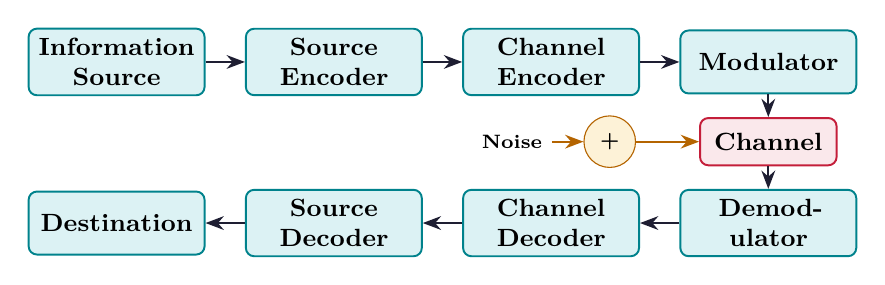
\begin{tikzpicture}[node distance=0.35cm and 0.55cm,
  sblock/.style={rectangle, draw=myteal, fill=hdrteal, text width=2.0cm,
    align=center, minimum height=0.8cm, font=\small\bfseries,
    rounded corners=3pt, line width=0.7pt}]
  
  % Row 1: Transmitter side
  \node[sblock] (src) {Information Source};
  \node[sblock, right=0.5cm of src] (senc) {Source Encoder};
  \node[sblock, right=0.5cm of senc] (cenc) {Channel Encoder};
  \node[sblock, right=0.5cm of cenc] (mod) {Modulator};
  
  % Row 2: Receiver side
  \node[sblock, below=1.2cm of mod] (demod) {Demodulator};
  \node[sblock, left=0.5cm of demod] (cdec) {Channel Decoder};
  \node[sblock, left=0.5cm of cdec] (sdec) {Source Decoder};
  \node[sblock, left=0.5cm of sdec] (dest) {Destination};

  % Middle block: Channel
  \path (mod.south) -- (demod.north) coordinate[midway] (chan_mid);
  \node[sblock, draw=myred, fill=hdrred, text width=1.5cm, minimum height=0.6cm] (chan) at (chan_mid) {Channel};

  % Arrows Row 1
  \draw[arrow] (src) -- (senc);
  \draw[arrow] (senc) -- (cenc);
  \draw[arrow] (cenc) -- (mod);
  \draw[arrow] (mod) -- (chan);

  % Arrows Row 2
  \draw[arrow] (chan) -- (demod);
  \draw[arrow] (demod) -- (cdec);
  \draw[arrow] (cdec) -- (sdec);
  \draw[arrow] (sdec) -- (dest);

  % Noise addition to channel
  \node[draw=myamber, fill=hdramber, circle, minimum size=0.4cm, left=0.8cm of chan, font=\scriptsize\bfseries] (sum) {+};
  \node[font=\scriptsize\bfseries, left=0.4cm of sum] (noise) {Noise};
  \draw[arrow, color=myamber] (noise) -- (sum);
  \draw[arrow, color=myamber] (sum) -- (chan);
\end{tikzpicture}
\end{tcolorbox}

\subsection{Measure of Information Content}
The "information" in a message is not related to its semantic meaning, but rather to its \textbf{uncertainty} or \textbf{surprise value}. An event that is highly likely to happen carries very little information when it occurs, whereas an extremely rare (unlikely) event carries high information.

\begin{tcolorbox}[defbox]
\textbf{Information Content:} The quantitative measure of the uncertainty associated with the occurrence of an event. For a discrete source emitting a symbol $x_i$ with probability $P(x_i)$, the information content $I(x_i)$ is inversely proportional to $P(x_i)$.
\end{tcolorbox}

\begin{tcolorbox}[formulabox, title={\textbf{Information Measurement Formula}}]
The information content $I(x_i)$ of symbol $x_i$ is defined as:
\begin{equation}
  I(x_i) = \log_r \left( \frac{1}{P(x_i)} \right) = -\log_r P(x_i)
\end{equation}
The unit of measurement depends on the base $r$ of the logarithm:
\begin{itemize}[leftmargin=1.5em, itemsep=2pt, topsep=2pt]
  \item[] \textbf{Base $r = 2$:} Units are \textbf{Bits} (Binary digits). $I(x_i) = -\log_2 P(x_i)$.
  \item[] \textbf{Base $r = e$:} Units are \textbf{Nats} (Natural units). $I(x_i) = -\ln P(x_i)$.
  \item[] \textbf{Base $r = 10$:} Units are \textbf{Hartleys} (or Decits). $I(x_i) = -\log_{10} P(x_i)$.
\end{itemize}
\textbf{Conversion Relations:}
\begin{align}
  1 \text{ Nat} &= \log_2 e \approx 1.443 \text{ Bits} \\
  1 \text{ Hartley} &= \log_2 10 \approx 3.322 \text{ Bits}
\end{align}
\end{tcolorbox}

\subsection{Entropy for Discrete Ensembles}
A discrete information source emits symbols from an alphabet $X = \{x_1, x_2, \dots, x_M\}$ with corresponding probabilities $P = \{P(x_1), P(x_2), \dots, P(x_M)\}$, where $\sum_{i=1}^M P(x_i) = 1$.

\begin{tcolorbox}[defbox]
\textbf{Entropy $H(X)$:} The average information content per symbol emitted by the source. It represents the mathematical expectation of the information of all symbols, measuring the overall uncertainty of the source.
\end{tcolorbox}

\begin{tcolorbox}[formulabox, title={\textbf{Entropy Formula}}]
\begin{equation}
  H(X) = E[I(x_i)] = \sum_{i=1}^M P(x_i) I(x_i) = -\sum_{i=1}^M P(x_i) \log_2 P(x_i) \quad (\text{bits/symbol})
\end{equation}
\end{tcolorbox}

\subsection{Properties of Entropy}
Entropy exhibits several fundamental properties that reflect its nature as a measure of uncertainty:

\begin{enumerate}[label=\textbf{\arabic*.}, leftmargin=*, itemsep=4pt]
  \item \textbf{Non-negativity:} $H(X) \ge 0$. Since $0 \le P(x_i) \le 1$, the term $-P(x_i) \log_2 P(x_i)$ is always non-negative.
  \item \textbf{Certainty (Minimum Entropy):} $H(X) = 0$ if and only if $P(x_i) = 1$ for some symbol $x_i$, and $P(x_j) = 0$ for all $j \ne i$. In this case, there is no uncertainty in the source output.
  \item \textbf{Maximality (Maximum Entropy):} $H(X) \le \log_2 M$, where $M$ is the number of symbols in the alphabet. The maximum uncertainty occurs when all symbols are equiprobable, i.e., $P(x_i) = 1/M$ for all $i$.
\end{enumerate}

\subsubsection{Derivation of Maximum Entropy Condition (Proof of Maximality)}
To find the probability distribution that maximizes $H(X)$ subject to the constraint $\sum_{i=1}^M P(x_i) = 1$, we use the method of Lagrange multipliers.
Let the objective function be:
\begin{equation*}
  f(P_1, P_2, \dots, P_M) = -\sum_{i=1}^M P_i \ln P_i
\end{equation*}
Subject to the constraint:
\begin{equation*}
  g(P_1, P_2, \dots, P_M) = \sum_{i=1}^M P_i - 1 = 0
\end{equation*}
Define the Lagrangian function $J$:
\begin{equation*}
  J = -\sum_{i=1}^M P_i \ln P_i - \lambda \left(\sum_{i=1}^M P_i - 1\right)
\end{equation*}
Differentiating $J$ with respect to $P_i$ and setting it to 0 for maximum value:
\begin{align*}
  \frac{\partial J}{\partial P_i} = - \ln P_i - 1 - \lambda &= 0 \\
  \ln P_i &= -(1 + \lambda) \\
  P_i &= e^{-(1+\lambda)}
\end{align*}
Since the right-hand side is constant and does not depend on the index $i$, all $P_i$ must be equal:
\begin{equation*}
  P_1 = P_2 = \dots = P_M = C \quad (\text{a constant})
\end{equation*}
Using the constraint $\sum_{i=1}^M P_i = 1$:
\begin{equation*}
  M \times C = 1 \implies C = \frac{1}{M} \implies P_i = \frac{1}{M} \quad \text{for all } i.
\end{equation*}
Substituting $P_i = 1/M$ back into the entropy formula yields the maximum entropy:
\begin{equation*}
  H(X)_{\text{max}} = -\sum_{i=1}^M \frac{1}{M} \log_2 \left(\frac{1}{M}\right) = -M \left(\frac{1}{M}\right) \left(-\log_2 M\right) = \log_2 M \quad \text{(Q.E.D.)}
\end{equation*}

\subsection{Binary Entropy Function}
For a binary source with alphabet $X = \{0, 1\}$ and probabilities $P(0) = p$ and $P(1) = 1-p$, the entropy is denoted by $H(p)$ or $H_b(p)$:
\begin{equation}
  H(p) = -p \log_2 p - (1-p) \log_2 (1-p)
\end{equation}

\begin{tcolorbox}[tikzbox, title={Binary Entropy Function $H(p)$ vs $p$}]
\centering
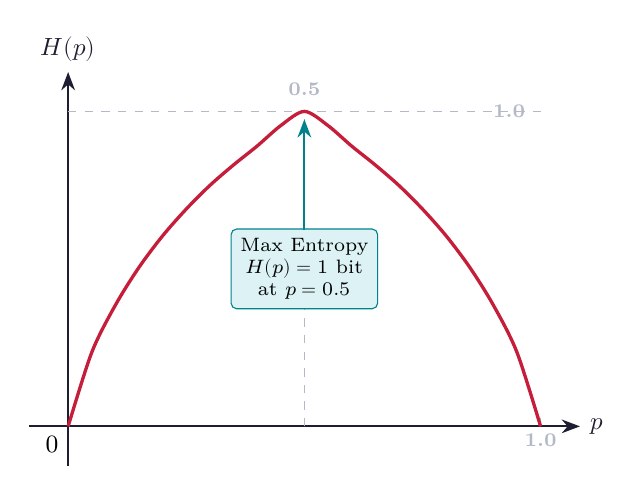
\begin{tikzpicture}
  % Draw axes
  \draw[-Stealth, thick, color=mydark] (-0.5,0) -- (6.5,0) node[right, font=\small] {$p$};
  \draw[-Stealth, thick, color=mydark] (0,-0.5) -- (0,4.5) node[above, font=\small] {$H(p)$};

  % Draw grid lines
  \draw[dashed, color=mgframe] (3,0) -- (3,4) node[above=2pt, font=\scriptsize\bfseries\color{mydark}] {0.5};
  \draw[dashed, color=mgframe] (0,4) -- (6,4) node[left=2pt, font=\scriptsize\bfseries\color{mydark}] {1.0};
  \draw[dashed, color=mgframe] (6,0) -- (6,0.1) node[below=2pt, font=\scriptsize\bfseries\color{mydark}] {1.0};

  % Plot the curve (manually plotting key points to avoid floating-point log domain errors)
  % Coordinates scaled: p=0 -> x=0, p=1 -> x=6; H(p)=0 -> y=0, H(p)=1 -> y=4
  \draw[very thick, color=myred, smooth] plot coordinates {
    (0.00, 0.00) (0.30, 0.94) (0.60, 1.54) (0.90, 2.02) (1.20, 2.42)
    (1.50, 2.76) (1.80, 3.06) (2.10, 3.32) (2.40, 3.56) (2.70, 3.82)
    (3.00, 4.00)
    (3.30, 3.82) (3.60, 3.56) (3.90, 3.32) (4.20, 3.06) (4.50, 2.76)
    (4.80, 2.42) (5.10, 2.02) (5.40, 1.54) (5.70, 0.94) (6.00, 0.00)
  };

  % Labels
  \node[below left, font=\small] at (0,0) {0};
  \node[draw=myteal, fill=hdrteal, rounded corners=2pt, font=\scriptsize, align=center] at (3,2) {Max Entropy\\$H(p) = 1$ bit\\at $p=0.5$};
  \draw[arrow, color=myteal] (3,2.5) -- (3,3.9);
\end{tikzpicture}
\end{tcolorbox}

% ===============================================================================
\section{Joint, Conditional, and Mutual Information}
% ===============================================================================

To analyze communication systems with an input source $X$ and an output destination $Y$, we define joint and conditional entropy metrics over the joint ensemble $(X, Y)$.

\subsection{Definitions of Entropies}
Let $P(x_i)$ be input probabilities, $P(y_j)$ be output probabilities, and $P(x_i, y_j)$ be the joint probability of transmitting $x_i$ and receiving $y_j$.

\begin{tcolorbox}[formulabox, title={\textbf{Joint and Conditional Entropies}}]
\begin{enumerate}[label=\textbf{\arabic*.}, leftmargin=1.5em, itemsep=4pt, topsep=2pt]
  \item \textbf{Joint Entropy $H(X, Y)$:} The total average uncertainty of the combined system.
    \begin{equation}
      H(X, Y) = -\sum_{i=1}^M \sum_{j=1}^N P(x_i, y_j) \log_2 P(x_i, y_j)
    \end{equation}
  \item \textbf{Conditional Entropy $H(X|Y)$:} The average uncertainty about the input $X$ after the output $Y$ is observed (also called \textbf{Equivocation}).
    \begin{equation}
      H(X|Y) = -\sum_{i=1}^M \sum_{j=1}^N P(x_i, y_j) \log_2 P(x_i|y_j)
    \end{equation}
  \item \textbf{Conditional Entropy $H(Y|X)$:} The average uncertainty about the output $Y$ when the input $X$ is known (represents the noise introduced by the channel).
    \begin{equation}
      H(Y|X) = -\sum_{i=1}^M \sum_{j=1}^N P(x_i, y_j) \log_2 P(y_j|x_i)
    \end{equation}
\end{enumerate}
\end{tcolorbox}

\subsubsection{Derivation of Joint Entropy Relations}
We derive the relation $H(X, Y) = H(X) + H(Y|X)$ using joint and conditional probability relationships $P(x_i, y_j) = P(x_i) P(y_j|x_i)$:
\begin{align*}
  H(X, Y) &= -\sum_{i=1}^M \sum_{j=1}^N P(x_i, y_j) \log_2 P(x_i, y_j) \\
  &= -\sum_{i=1}^M \sum_{j=1}^N P(x_i, y_j) \log_2 \left[ P(x_i) P(y_j|x_i) \right] \\
  &= -\sum_{i=1}^M \sum_{j=1}^N P(x_i, y_j) \left[ \log_2 P(x_i) + \log_2 P(y_j|x_i) \right] \\
  &= -\sum_{i=1}^M \left( \sum_{j=1}^N P(x_i, y_j) \right) \log_2 P(x_i) - \sum_{i=1}^M \sum_{j=1}^N P(x_i, y_j) \log_2 P(y_j|x_i)
\end{align*}
Using the probability marginalization rule $\sum_{j=1}^N P(x_i, y_j) = P(x_i)$:
\begin{equation*}
  H(X, Y) = -\sum_{i=1}^M P(x_i) \log_2 P(x_i) + H(Y|X) = H(X) + H(Y|X) \quad \text{(Q.E.D.)}
\end{equation*}
Similarly, using $P(x_i, y_j) = P(y_j) P(x_i|y_j)$, we can prove:
\begin{equation}
  H(X, Y) = H(Y) + H(X|Y)
\end{equation}

\subsection{Mutual Information}
\begin{tcolorbox}[defbox]
\textbf{Mutual Information $I(X; Y)$:} The amount of information about the source $X$ that is obtained by observing the channel output $Y$. It measures the reduction in uncertainty of $X$ due to the knowledge of $Y$.
\end{tcolorbox}

\begin{tcolorbox}[formulabox, title={\textbf{Mutual Information Formulas}}]
\begin{equation}
  I(X; Y) = H(X) - H(X|Y) \quad (\text{bits/symbol})
\end{equation}
By symmetry and joint entropy relations, it can also be expressed as:
\begin{align}
  I(X; Y) &= H(Y) - H(Y|X) \\
  I(X; Y) &= H(X) + H(Y) - H(X, Y)
\end{align}
In terms of probabilities:
\begin{equation}
  I(X; Y) = \sum_{i=1}^M \sum_{j=1}^N P(x_i, y_j) \log_2 \left[ \frac{P(x_i, y_j)}{P(x_i)P(y_j)} \right]
\end{equation}
\end{tcolorbox}

\subsection{Properties of Mutual Information}
\begin{itemize}[leftmargin=*, itemsep=3pt]
  \item \textbf{Symmetry:} $I(X; Y) = I(Y; X)$. The channel output $Y$ carries the same amount of information about the input $X$ as the input $X$ carries about the output $Y$.
  \item \textbf{Non-negativity:} $I(X; Y) \ge 0$. The observation of $Y$ can never increase the uncertainty of $X$ on average.
  \item \textbf{Independence Condition:} $I(X; Y) = 0$ if and only if $X$ and $Y$ are statistically independent. In this case, receiving $Y$ provides no information about $X$.
  \item \textbf{Relation to Channel Capacity:} For deterministic, noiseless channels, conditional uncertainty vanishes, and $I(X; Y) = H(X)$.
\end{itemize}

\subsection{Entropy Relationship Diagram}
The relationships between all these entropy measures are summarized in the Venn diagram below:

\begin{tcolorbox}[tikzbox, title={Venn Diagram of Entropy Relationships}]
\centering
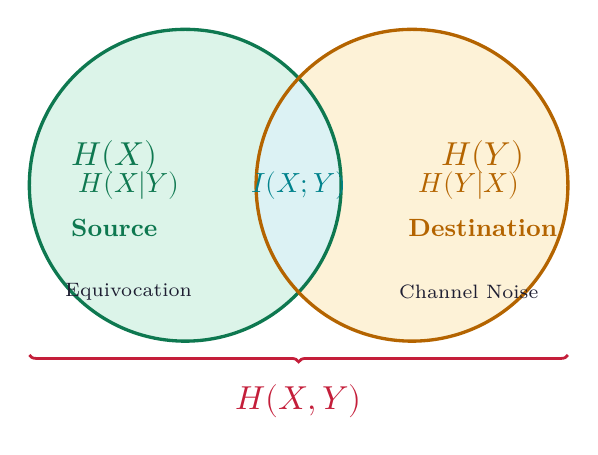
\begin{tikzpicture}[thick, scale=0.9]
  % Define overlapping circles
  \def\circleA{(-1.6,0) circle (2.2cm)}
  \def\circleB{(1.6,0) circle (2.2cm)}

  % Fill colors
  \begin{scope}
    \clip \circleA;
    \fill[hdrteal] \circleB; % Intersection (Mutual Info)
  \end{scope}

  \begin{scope}
    \clip \circleA;
    \fill[hdrgreen] \circleA;
    \clip \circleB;
    \fill[hdrteal] \circleA; % Redo intersection to keep clean
  \end{scope}
  
  \begin{scope}
    \clip \circleB;
    \fill[hdramber] \circleB;
    \clip \circleA;
    \fill[hdrteal] \circleB;
  \end{scope}

  % Draw outlines of circles
  \draw[mygreen, line width=1.2pt] \circleA;
  \draw[myamber, line width=1.2pt] \circleB;

  % Set labels
  \node[font=\large\bfseries\color{mygreen}] at (-2.6, 0.4) {$H(X)$};
  \node[font=\large\bfseries\color{myamber}] at (2.6, 0.4) {$H(Y)$};

  \node[font=\small\bfseries\color{mygreen}] at (-2.6, -0.6) {Source};
  \node[font=\small\bfseries\color{myamber}] at (2.6, -0.6) {Destination};

  % Labels inside divisions
  \node[font=\normalsize\bfseries\color{mygreen}] at (-2.4, 0) {$H(X|Y)$};
  \node[font=\normalsize\bfseries\color{myamber}] at (2.4, 0) {$H(Y|X)$};
  \node[font=\normalsize\bfseries\color{myteal}] at (0, 0) {$I(X; Y)$};

  % Curly brace for joint entropy
  \draw[decoration={brace, mirror, raise=5pt}, decorate, color=myred, line width=1pt] 
    (-3.8,-2.2) -- (3.8,-2.2) node[midway, below=12pt, font=\large\bfseries\color{myred}] {$H(X, Y)$};

  % Details below
  \node[font=\scriptsize\color{mydark}] at (-2.4,-1.5) {Equivocation};
  \node[font=\scriptsize\color{mydark}] at (2.4,-1.5) {Channel Noise};
\end{tikzpicture}
\end{tcolorbox}

% ===============================================================================
\section{Shannon's First Theorem \& Source Coding}
% ===============================================================================

Source coding is the process of representing discrete source symbols with binary code words. The goal is to reduce data size by removing redundancy.

\subsection{Shannon's Noiseless Coding Theorem}
\begin{tcolorbox}[defbox]
\textbf{Shannon's First Theorem (Source Coding Theorem):} For a discrete memoryless source $X$ with entropy $H(X)$ (bits/symbol), the average codeword length $L$ (bits/symbol) for any uniquely decodable binary code is bounded by:
\begin{equation}
  L \ge H(X)
\end{equation}
By coding sequences of $N$ symbols at a time (block coding), the average code length per source symbol $L_N$ can be made arbitrarily close to $H(X)$ as $N \to \infty$:
\begin{equation}
  \lim_{N \to \infty} L_N = H(X)
\end{equation}
\end{tcolorbox}

\subsection{Performance Metrics of Source Codes}
For a source emitting symbols $s_i$ with probability $P(s_i)$ and assigned codeword length $l_i$ (in bits):
\begin{tcolorbox}[formulabox, title={\textbf{Average Length, Efficiency, and Redundancy}}]
\begin{enumerate}[label=\textbf{\arabic*.}, leftmargin=1.5em, itemsep=4pt, topsep=2pt]
  \item \textbf{Average Codeword Length ($L$):}
    \begin{equation}
      L = \sum_{i=1}^M P(s_i) l_i \quad (\text{bits/symbol})
    \end{equation}
  \item \textbf{Coding Efficiency ($\eta$):}
    \begin{equation}
      \eta = \frac{H(X)}{L} \times 100\%
    \end{equation}
  \item \textbf{Code Redundancy ($R$):}
    \begin{equation}
      R = 1 - \eta = 1 - \frac{H(X)}{L}
    \end{equation}
\end{enumerate}
\end{tcolorbox}

\subsection{Prefix Codes and Kraft-McMillan Inequality}
A code is \textbf{uniquely decodable} if any concatenated sequence of codewords can be decoded in only one way.
\begin{tcolorbox}[defbox]
\textbf{Prefix Code (Instantaneous Code):} A uniquely decodable code with the property that no codeword is a prefix of any other codeword. This allows a sequence to be decoded symbol-by-symbol instantaneously as it is received, without waiting for the end of the sequence.
\end{tcolorbox}

\begin{tcolorbox}[formulabox, title={\textbf{Kraft-McMillan Inequality}}]
A prefix code (or any uniquely decodable code) with alphabet size $D$ (usually binary, $D=2$) and codeword lengths $l_1, l_2, \dots, l_M$ exists if and only if:
\begin{equation}
  \sum_{i=1}^M D^{-l_i} \le 1
\end{equation}
For binary codes, this is:
\begin{equation}
  \sum_{i=1}^M 2^{-l_i} \le 1
\end{equation}
If the inequality is satisfied with equality ($\sum 2^{-l_i} = 1$), the code is called a \textbf{complete code} (no further codewords can be added without violating the prefix property).
\tcbset{colbacktitle=myteal, coltitle=white}
\end{tcolorbox}

\subsection{Shannon-Fano Coding Algorithm}
Shannon-Fano coding is a top-down algorithm to construct prefix codes. The procedure is:
\begin{enumerate}[label=\textbf{Step \arabic*:}, leftmargin=4.5em, itemsep=3pt]
  \item Sort the source symbols in descending order of their probabilities.
  \item Divide the sorted list of symbols into two subsets such that the sum of probabilities of the two subsets is as close to equal as possible.
  \item Assign binary code '0' to all symbols in the first (upper) subset and '1' to all symbols in the second (lower) subset.
  \item Recursively apply Steps 2 and 3 to each subset until each sub-sublist contains exactly one symbol.
  \item The codeword for each symbol is the sequence of 0s and 1s assigned to it from the root of divisions.
\end{enumerate}

\begin{tcolorbox}[examplebox, title={Worked Example: Shannon-Fano Coding}]
\textbf{Problem:} A discrete memoryless source emits 5 symbols $\{s_1, s_2, s_3, s_4, s_5\}$ with probabilities $P = \{0.35, 0.30, 0.20, 0.10, 0.05\}$. 
\begin{enumerate}[label=\alph*., leftmargin=*, itemsep=1pt, topsep=1pt]
  \item Construct a binary Shannon-Fano code.
  \item Calculate the entropy $H(X)$ of the source.
  \item Calculate the average codeword length $L$ and the efficiency $\eta$.
\end{enumerate}
\textbf{Solution:}

\textbf{(a) Code Construction Table:}\par\noindent
\begin{tabularx}{\linewidth}{|B{1.5cm}|Y|Y|Y|Y|B{2.2cm}|B{1.6cm}|}
\hline
\textbf{Symbol} & \textbf{Prob.} & \textbf{Stage 1} & \textbf{Stage 2} & \textbf{Stage 3} & \textbf{Codeword} & \textbf{Length ($l_i$)} \\
\hline
$s_1$ & 0.35 & 0 & 0 & & 00 & 2 \\
$s_2$ & 0.30 & 0 & 1 & & 01 & 2 \\
\hline
$s_3$ & 0.20 & 1 & 0 & & 10 & 2 \\
$s_4$ & 0.10 & 1 & 1 & 0 & 110 & 3 \\
$s_5$ & 0.05 & 1 & 1 & 1 & 111 & 3 \\
\hline
\end{tabularx}
\par\vspace{4pt}
\textit{Division Rationale:}
\begin{itemize}[leftmargin=*, itemsep=1pt]
  \item \textbf{Stage 1:} Split between $\{s_1, s_2\}$ (sum = 0.65) and $\{s_3, s_4, s_5\}$ (sum = 0.35). Difference is $0.30$. (Splitting between $s_1$ and others yields difference $0.35 - 0.65 = 0.30$, so both partitions are valid. Let's use the first).
  \item \textbf{Stage 2:} Split upper subset $\{s_1\}$ (0.35) and $\{s_2\}$ (0.30). Split lower subset $\{s_3\}$ (0.20) and $\{s_4, s_5\}$ (0.15).
  \item \textbf{Stage 3:} Split $\{s_4\}$ (0.10) and $\{s_5\}$ (0.05).
\end{itemize}

\textbf{(b) Source Entropy $H(X)$:}
\begin{align*}
  H(X) &= -\sum_{i=1}^5 P(s_i) \log_2 P(s_i) \\
  &= -[0.35\log_2 0.35 + 0.30\log_2 0.30 + 0.20\log_2 0.20 + 0.10\log_2 0.10 + 0.05\log_2 0.05] \\
  &= -[0.35(-1.5146) + 0.30(-1.7370) + 0.20(-2.3219) + 0.10(-3.3219) + 0.05(-4.3219)] \\
  &= -[-0.5301 - 0.5211 - 0.4644 - 0.3322 - 0.2161] = 2.0639 \text{ bits/symbol}
\end{align*}

\textbf{(c) Average Codeword Length $L$ and Efficiency $\eta$:}
\begin{align*}
  L &= \sum_{i=1}^5 P(s_i) l_i = (0.35 \times 2) + (0.30 \times 2) + (0.20 \times 2) + (0.10 \times 3) + (0.05 \times 3) \\
  &= 0.70 + 0.60 + 0.40 + 0.30 + 0.15 = 2.15 \text{ bits/symbol} \\[4pt]
  \eta &= \frac{H(X)}{L} \times 100\% = \frac{2.0639}{2.15} \times 100\% \approx 95.99\% \\[4pt]
  \text{Redundancy } R &= 1 - 0.9599 = 0.0401 \text{ or } 4.01\%
\end{align*}
\textbf{Kraft Inequality Verification:}
\begin{equation*}
  \sum_{i=1}^5 2^{-l_i} = 2^{-2} + 2^{-2} + 2^{-2} + 2^{-3} + 2^{-3} = 0.25 + 0.25 + 0.25 + 0.125 + 0.125 = 1.0 \le 1
\end{equation*}
The sum equals 1.0. This indicates that the code is prefix-free and is a complete code.
\end{tcolorbox}

% ===============================================================================
% MANDATORY QUICK REVISION PAGE
% ===============================================================================
\newpage
\begin{center}
  {\large\bfseries\color{myred} Quick Revision --- Module I}\\[3pt]
  {\small\color{mydark} Basics \& Source Coding $|$ PE-EC603D}
\end{center}
\noindent{\color{myred}\rule{\linewidth}{1.2pt}}
\vspace{4pt}

\begin{tcolorbox}[formulabox, title={\textbf{Key Formulas at a Glance}}]
\renewcommand{\arraystretch}{1.3}
\begin{tabularx}{\linewidth}{B{4.5cm} X}
Self-Information        & $I(x_i) = \log_2 \left( \frac{1}{P(x_i)} \right) = -\log_2 P(x_i)$ \\[4pt]
Entropy (Average Info)   & $H(X) = -\sum_{i=1}^M P(x_i) \log_2 P(x_i)$ \\[4pt]
Joint Entropy           & $H(X, Y) = -\sum \sum P(x_i, y_j) \log_2 P(x_i, y_j)$ \\[4pt]
Conditional Entropies   & $H(X|Y) = H(X, Y) - H(Y)$ \quad and \quad $H(Y|X) = H(X, Y) - H(X)$ \\[4pt]
Mutual Information      & $I(X; Y) = H(X) - H(X|Y) = H(Y) - H(Y|X)$ \\[4pt]
Average Code Length     & $L = \sum P(s_i) l_i$ \\[4pt]
Coding Efficiency       & $\eta = \frac{H(X)}{L} \times 100\%$ \\[4pt]
Kraft Inequality        & $\sum 2^{-l_i} \le 1 \quad (\text{For binary prefix codes})$
\end{tabularx}
\end{tcolorbox}

\begin{tcolorbox}[defbox, title={\textbf{One-Line Definitions}}]
\begin{itemize}[leftmargin=*, itemsep=2.5pt, topsep=0pt]
  \item \textbf{Information Content:} A measure of surprise or uncertainty of an event, dependent only on its probability.
  \item \textbf{Entropy:} The average uncertainty or information content per symbol emitted by a source.
  \item \textbf{Equivocation $H(X|Y)$:} The residual uncertainty of the input $X$ after output $Y$ is observed at the receiver.
  \item \textbf{Mutual Information:} The amount of information shared between the transmitter and receiver.
  \item \textbf{Prefix Code:} A code in which no codeword is a prefix of another, enabling instantaneous decoding.
  \item \textbf{Kraft Inequality:} A mathematical condition determining the existence of prefix codes for given lengths.
  \item \textbf{Source Coding Theorem:} Shannon's limit stating that average codeword length cannot be less than source entropy.
  \item \textbf{Redundancy:} The percentage of code space wasted by transmitting non-informative bits ($R = 1 - \eta$).
\end{itemize}
\end{tcolorbox}

\begin{tcolorbox}[exambox, title={\textbf{Frequently Asked / Viva Questions}}]
\begin{enumerate}[topsep=0pt, label=\textbf{Q\arabic*.}, itemsep=5pt]
  \item \Q{State the units of information and their conversion relations.}
    Bits (base 2), Nats (base $e$), and Hartleys (base 10). Conversions: $1 \text{ Nat} = 1.443 \text{ Bits}$; $1 \text{ Hartley} = 3.322 \text{ Bits}$.
  \item \Q{Under what condition is the entropy of a source maximized?}
    When all $M$ symbols of the source alphabet are equiprobable, i.e., $P(x_i) = 1/M$ for all $i$. The maximum entropy is $H(X)_{\text{max}} = \log_2 M$.
  \item \Q{What is the physical significance of conditional entropy $H(Y|X)$?}
    It represents the average uncertainty of the output $Y$ when the input $X$ is known. Physically, it measures the noise added by the channel.
  \item \Q{Explain the term "Equivocation" in communication channels.}
    Equivocation is $H(X|Y)$, which is the average uncertainty about the transmitted symbol $X$ after receiving symbol $Y$. It represents lost information.
  \item \Q{Why is Mutual Information symmetric?}
    $I(X; Y) = I(Y; X) = H(X) + H(Y) - H(X,Y)$. It represents the shared information between $X$ and $Y$, making the direction of analysis irrelevant.
  \item \Q{State Shannon's Source Coding Theorem.}
    The average length $L$ of any uniquely decodable binary code for a source $X$ satisfies $L \ge H(X)$. The minimum average code length is limited by the source entropy.
  \item \Q{What is an instantaneous code (prefix code)?}
    A code where no codeword is a prefix of any other codeword. It is decodable immediately upon receiving the last bit of the codeword, without looking ahead.
  \item \Q{What is the significance of the Kraft-McMillan Inequality?}
    It provides a necessary and sufficient condition for the existence of an instantaneous (prefix) code for a given set of codeword lengths.
  \item \Q{If a source has an entropy of $1.8$ bits/symbol and is encoded using a code with average length $2$ bits/symbol, find efficiency and redundancy.}
    Efficiency $\eta = \frac{1.8}{2} \times 100 = 90\%$. Redundancy $R = 100\% - 90\% = 10\%$.
  \item \Q{Why does block coding increase source coding efficiency?}
    Block coding groups $N$ symbols together, allowing the average length per symbol to approach the entropy $H(X)$ more closely as $N \to \infty$ by utilizing joint probabilities.
  \item \Q{Can the efficiency of a source code be greater than $100\%$?}
    No. According to Shannon's Source Coding Theorem, $L \ge H(X)$, meaning efficiency $\eta = H(X)/L \le 1.0$ (or $100\%$).
  \item \Q{State the main difference between Shannon-Fano and Huffman coding approaches.}
    Shannon-Fano is a top-down approach that partitions probabilities into subgroups, while Huffman coding is a bottom-up approach that recursively merges the lowest probabilities.
\end{enumerate}
\end{tcolorbox}

\begin{tcolorbox}[tikzbox, title={Comparison of Source Coding Techniques}]
\renewcommand{\arraystretch}{1.4}
\par\noindent
\begin{tabularx}{\linewidth}{|B{3.2cm}|Y|Y|}
\hline
\textbf{Parameter} & \textbf{\color{myteal}Fixed-Length Coding} & \textbf{\color{mygreen}Variable-Length Coding} \\
\hline
\textbf{Codeword Length} & Equal length ($l_i = \lceil \log_2 M \rceil$) for all symbols. & Different lengths based on symbol probabilities. \\
\hline
\textbf{Probability Sensitivity} & Ignores probability distribution. & Allocates shorter codes to high-probability symbols. \\
\hline
\textbf{Efficiency} & Low if symbols have unequal probabilities. & High (approaches Shannon's limit $H(X)$). \\
\hline
\textbf{Synchronization} & Easy; boundaries are known. & Harder; requires prefix-free property (Prefix codes). \\
\hline
\textbf{Examples} & ASCII, Standard PCM. & Shannon-Fano, Huffman coding. \\
\hline
\end{tabularx}
\end{tcolorbox}

\end{document}
